%
% numerik.tex -- numerische Lösung von gewöhnlichen Differentialgleichungen
%
% (c) 2015 Prof Dr Andreas Mueller, Hochschule Rapperswil
%
\chapter{Numerische L"osung\label{chapter:numerik}}
\lhead{}
\rhead{Numerische L"osung}
\index{Numerische Loesung@Numerische L\"osung}
Im Kapitel~\ref{chapter:grundlagen} waren wir in der Lage, f"ur einige
einfache Differentialgleichungen eine L"osung in geschlossener Form
zu finden.
Zum Beispiel konnten wir lineare Differentialgleichungen mit Hilfe
der Exponentialfunktion l"osen.
Dieses Bild tr"ugt allerdings.
Die meisten Differentialgleichungen k"onnen nicht in geschlossener
Form gel"ost werden.
Wir k"onnen daher nicht erwarten, dass wir die L"osungen beliebiger
Differentialgleichungen einfach dadurch verstehen, dass wir
L"osungsfunktionen diskutieren.
Stattedessen bleiben uns nur die folgenden zwei M"oglichkeiten:
\begin{enumerate}
\item
Wir l"osen die Differentialgleichung mit Hilfe eines Computers,
und studieren den Verlauf der L"osungsfunktionen oder die Abh"angigkeit
von Parameter oder Anfangsbedingungen durch Vergleich verschiedener
numerisch gefundener L"osungen.
\item
Wir entwickeln Methoden, mit denen sich Aussagen "uber den Verlauf der
L"osungskurven studieren lassen, ohne dass man sie berechnet haben muss.
Nat"urlich kann man nicht erwarten, dass eine solche Methode genaue
Aussagen dar"uber erlaubt, wann eine L"osungskurve wo genau durchgehen
wird.
Es werden nur qualititative Aussagen m"oglich sein, zum Beispiel ob
Gleichgewichtsl"osunge stabil sind, ob es periodische L"osungen gibt
und ob L"osungskurven zu den periodischen L"osungen konvergieren.
\end{enumerate}
In diesem Kapitel entwickeln wir Methoden, Differentialgleichungen 
numerisch zu l"osen.

\section{Grundprinzip}
\lhead{Grundprinzip}
\begin{figure}
\centering
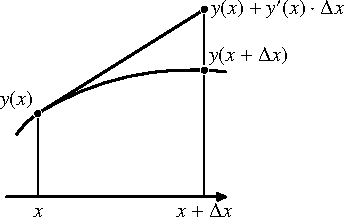
\includegraphics{chapters/images/numerik-2.pdf}
\caption{Lineare Approximation von $y(x+\Delta x)$ durch Information,
die am Punkt $x$ verf"ugbar ist.
\label{numerik:lineareapproximation}}
\end{figure}
Wir versuchen die Differentialgleichung
\begin{equation}
y'=-\alpha y,\qquad y(0)=y_0
\label{numerik:expdgl}
\end{equation}
numerisch zu l"osen. 
Dazu unterteilen wir die $x$-Achse in diskrete Abschnitte der L"ange $h$,
und bezeichnen die Teilpunkte mit $x_k=kh$.
Das Ziel ist jetzt, $y(x_k)$ n"aherungsweise zu berechnen.
Wir schreiben $y_k$ f"ur die N"aherungswerte von $y(x_k)$.
Die Ableitung liefert eine lineare Approximation f"ur $y(x)$,
n"amlich
\[
y(x+\Delta x)\simeq y(x) + y'(x)\cdot\Delta x
\]
(Abbildung~\ref{numerik:lineareapproximation}).
F"ur die Punkte $x_k$ bedeutet das
\[
y(x_{k+1})\simeq y(x_{k})+y'(x_k)\dot h.
\]
Die Differentialgleichung liefert Werte f"ur $y'(x_k)$ aus $x_k$ und $y(x_k)$,
damit k"onnen wir aus dieser Approximation ein allgemeines
N"aherungsverfahren f"ur die L"osung einer Differentialgleichung
konstruieren.

\begin{satz}[Euler-Verfahren]
\index{Euler-Verfahren}
Die Differentialgleichung
\begin{equation}
y'=f(x,y),\qquad y(0)=y_0
\label{numerik:eulerdgl}
\end{equation}
und die Schrittweite $h$ definieren eine Folge 
\[
y_{\mathstrut k}=y_{k-1} + h\cdot f(x_{k-1}, y_{k-1}),\quad k>0,
\]
mit $x_k=kh$,
die eine N"aherung f"ur die Funktionswerte $y(x_k)$ der L"osung $y(x)$
der Differentialgleichung~(\ref{numerik:eulerdgl}) ist.
\end{satz}

Dieses Verfahren ist nicht besonders gut, wie wir im Folgenden zeigen
wollen.
Die Diskussion soll uns aber zeigen, worauf bei der Weiterentwicklung
des Verfahrens geachtet werden muss.

Im vorliegenden Beispiel liefert die
Differentialgleichung~(\ref{numerik:expdgl})
den Wert $y'(x_k)=-\alpha y(x_k)$ f"ur die Ableitung,
woraus wir die Rekursionsformel
\[
y_{k+1}=y_k - \alpha y_k \dot h.
\]
gewinnen.
Die Rekursionsgleichung kann in diesem Fall exakt gel"ost werden,
und wir finden
\begin{equation}
y(x_{k+1}) = y(x_k)-\alpha y(x_k) h=(1-\alpha h) y(x_k)=\dots
=(1-\alpha h)^{k+1}y_0
\label{numerik:rekursion}
\end{equation}
f"ur die N"aherung $y_k$ der Funktionswerte $y(x_k)$.
%Angewendet auf eine beliebige Differentialgleichung, ist dieses
%einfache numerische Verfahren bekannt als das {\em Euler-Verfahren}.
%Es ist nicht besonders genau, aber soll in diesem Abschnitt dazu
%dienen, die Anforderungen an ein gutes numerisches Verfahren
%zu illustrieren.



Wir m"ochten $y(x)$ f"ur einen ganz bestimmten $x$-Wert berechnen.
Dazu unterteilen wir das Interval $[0,x]$ in $n$ Teilschritte der
Breite $x/n$, und wenden die Formel~(\ref{numerik:rekursion}) an:
\[
y(x)=y(x_n)=(1-\alpha h)^n y_0=\biggl(1+\frac{-\alpha x}{n}\biggr)^n y_0.
\]
F"ur eine grosse Zahl von Teilschritten erhalten wir so tats"achlich die
korrekte L"osung:
\[
\lim_{n\to\infty}y_0\biggl(1+\frac{-\alpha x}n\biggr)^n=y_0 e^{-\alpha x}.
\]
\begin{figure}
\centering
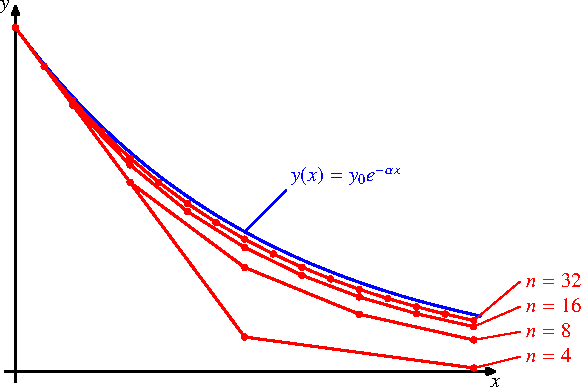
\includegraphics{chapters/images/numerik-1.pdf}
\caption{Approximationen der L"osung der Differentialgleichung $y'=-\alpha y$
mit verschiedener Anzahl Schritte (rot) n"ahern sich f"ur wachsendes
$n$ der exakten L"osung (blau).
\label{numerik:approximation}}
\end{figure}%
Abbildung~\ref{numerik:approximation} zeigt, wie die
durch~(\ref{numerik:rekursion}) gegebenen Approximationen mit zunehmendem
$n$ der exakten L"osung $y(x)=e^{-\alpha x}$ n"aher kommen.

Wir k"onnen auch den Fehler des numerischen Verfahrens berechnen.
Bei der Schrittweite $h$ ist der Fehler von $y_k$ die Differenz
\[
y(x_k)-y_k
=
y_0e^{-\alpha kh}-y_0(1-\alpha h)^k
=
y_0((e^{-\alpha h})^k - (1-\alpha h)^k)
=
y_0e^{-\alpha hk}\biggl(
1-\biggl(\frac{1-\alpha h}{e^{-\alpha h}}\biggr)^k
\biggr).
\]
Man beachte, dass der Z"ahler $1-\alpha h$ die Approximation
$y_1$ ist, als eine Approximation von $e^{-\alpha h}$, dem Nenner.
Schreiben wir
\[
q=\frac{1-\alpha h}{e^{-\alpha h}},
\]
f"ur den Quotienten zwischen der Approximation und dem korrekten Wert,
dann ist sicher immer $q<1$.
Den Fehler k"onnen wir jetzt schreiben
\[
y(x_k)-y_k = y_0e^{-\alpha hk}(1-q^k) = y(x_k)(1-q^k).
\]
Der relative Fehler des Verfahrens ist also
\[
\frac{y(x_k)-y_k}{y(x_k)}=(1-q^k).
\]
\begin{figure}
\centering
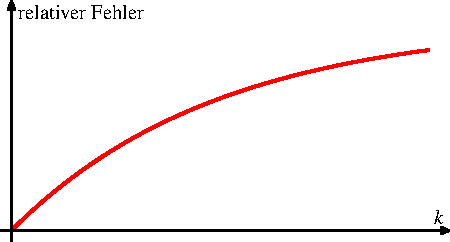
\includegraphics{chapters/images/numerik-3.pdf}
\caption{Relativer Fehler des Eulerverfahrens f"ur die Differentialgleichung
(\ref{numerik:expdgl}) in Abh"angigkeit von der Anzahl $k$ der Schritte.
\label{numerik:relfehler}}
\end{figure}%
Ganz unabh"angig von der Schrittweite $h$ wird der relative Fehler
des Verfahrens immer gegen 1 streben, der Fehler wird also von der
gleichen Gr"ossenordnung wie die berechneten Resultate.

Die Abbildung~\ref{numerik:relfehler} zeigt, dass zu Beginn des Verfahrens
der relative Fehler ungef"ahr linear mit der Anzahl der Schritt zunimmt.
Um eine angemessene Genauigkeit "uber einen gr"osseren Bereich
zu erreichen, muss das Euler-Verfahren also sehr viel kleinere Schritte
und eine entsprechend gr"ossere Anzahl von Schritten ausf"uhren,
die entsprechend viel Rechenzeit ben"otigen.

Ein praktisch n"utzliches Verfahren muss also anstreben, mit einer
sehr viel kleineren Anzahl von Schritten eine viel gr"ossere Genaugikeit
der Approximations zu erreichen.

\section{Fehler-Entwicklung numerischer L"osungen}
\lhead{Fehler-Entwicklung}
Wir betrachten wieder die Differentialgleichung~(\ref{numerik:eulerdgl})
und versuchen, den Fehler eines N"aherungsverfahrens zu bestimmen,
welches Schritte der Gr"osse $h$ durchf"uhrt, um den Wert $y(x)$
zu approximieren.

Das Euler-Verfahren verwendet Schritte der Form
\[
y_{k+1}=y_{k\mathstrut} + hf(x_{k\mathstrut},y_{k\mathstrut}).
\]
In jedem einzelnen Schritt entsteht ein Fehler, dessen Gr"osse wir
aus der Taylor-Entwicklung
\[
y(x+\Delta x)=
y(x) + y'(x)\cdot \Delta x + R(x) \Delta x^2
\]
absch"atzen k"onnen.
Die Funktion $R(x)$ ist beschr"ankt und beschreibt den verbleibenden
Fehler.
Um $y(x)$ zu approximieren, m"ussen $n=x/h$ Schritte der Schrittweite
$h$ durchgef"uhrt werden, von denen jeder einen Fehler
von der Gr"ossenordnung $R(x)h^2$ hat.
Der Gesamtfehler ist daher von der Gr"ossenordnung
\[
y(x)-y_n=O\biggl(R(x)h^2\frac{x}h\biggr)=O(h),
\]
er ist also von erster Ordnung in $h$.
Um eine zus"atzliche Stelle Genauigkeit zu erhalten, muss man also zehnmal
so viele Schritte von zehnmal kleinerer Gr"osse durchf"uhren,
wodurch auch wieder Rundungsfehler eingef"uhrt werden.

K"onnte man den Fehler des Einzelschrittes wesentlich verkleinern, w"urde
auch die Abh"angigkeit des Fehlers des Verfahrens vorteilhafter.
W"are der Fehler des Einzelschrittes $O(h^k)$ statt $O(h^2)$, dann
w"are der Gesamtfehler des Verfahrens nur noch $O(h^{k-1})$.
F"ur $k=3$ bedeutet dies, dass eine Halbierung der Schrittweite
zwar doppelt so viele Schritte braucht, aber auch, dass in jedem
Schritt nur ein Achtel des Fehlers auftritt.
Der Gesamtfehler ist also nur ein Viertel.
Mit zehnmal mehr Arbeit kann man also nicht nur eine Stelle an
Genauigkeit gewinnen, sondern gleich deren zwei.

Man nennt ein Verfahren, bei dem der Gesamt-Fehler von der Gr"ossenordnung
$O(h^k)$ ist, von einem Verfahren $k$-ter Ordnung.
Das Euler-Verfahren ist also ein Verfahren erster Ordnung oder ein
lineares Verfahren.
In der Praxis werden Verfahren bis zu vierter und f"unfter Ordnung
verwendet, so dass eine zehnmal kleinere Schrittweite zu gleich
vier Stellen Genauigkeitsgewinn f"uhren.
Das Ziel der kommenden Abschnitte muss daher sein, einfach
berechnebare Approximationen der Funktion mit m"oglichst geringen
Einzelschrittfehlern zu finden.

\section{Einschritt-Verfahren\label{section:numerik:einschritt}}
\lhead{Einschritt-Verfahren}
Die relativ geringe Genauigkeit des Eulerschrittes beruht darauf,
dass die zu Beginn des Schrittes berechnete Ableitung $f(x_k,y_k)$
nur f"ur das linke Ende des Intervals $[x_k, x_k+h]$ zutrifft,
weiter rechts im Interval wird die Abweichung immer gr"osser.
Eine m"ogliche L"osung des Problems k"onnte darin bestehen, statt
nur einer linearen N"aherung zus"atzliche Glieder der Taylorreihe
\begin{equation}
y(x+\Delta x)
=
y(x)
+
y'(x)\cdot \Delta x
+
\frac12 y''(x)\cdot \Delta x^2
+
\frac16 y'''(x)\cdot \Delta x^3
+
o(\Delta x^3)
\label{numerik:taylor}
\end{equation}
zu verwenden.
In (\ref{numerik:taylor}) werden h"ohere Ableitungen von $y(x)$ ben"otigt,
w"ahrend die Differentialgleichung nur die erste Ableitung liefert.
Die h"oheren Ableitungen wurden aber bereits im
Abschnitt~\ref{grundlagen:hoehere-ableitungen} berechnet.

Wir untersuchen, wie sich das Verfahren f"ur die Beispiel-Gleichung
(\ref{numerik:expdgl}) anwenden l"asst.
Dort gilt
\begin{equation*}
\begin{aligned}
y'(x)&=f(x,y)=-\alpha y
\\
\Rightarrow\qquad
\frac{\partial f}{\partial x}&=0&\frac{\partial f}{\partial y}&=-\alpha
\end{aligned}
\end{equation*}
Alle zweiten Ableitungen verschwinden.
Die Gleichungen werden damit einfach:
\begin{align*}
y''(x)&=-\alpha f(x,y)=\alpha^2 y
\\
y'''(x)&=\alpha^2f(x,y)=-\alpha^3 y.
\end{align*}
Statt der linearen Approximation sollte daher die kubische Approximation
\begin{equation}
y_{k+1}
=
y_{k}-\alpha h y_k +\frac12\alpha^2 h^2 y_k -\frac16 \alpha^3h^3 y_k
=
y_{k}\underbrace{\biggl(1-\alpha h +\frac12\alpha^2h^2 -\frac16 \alpha^3h^3\biggr)}_{\simeq e^{-\alpha h}}
\label{numerik:kubisch}
\end{equation}
verwendet werden.
Dass man hier mit einer gr"osseren Genauigkeit rechnen darf ist schon daran
erkennbar, dass der Klammerausdruck auf der rechten Seite eine viel
bessere Approximation von $e^{-\alpha x}$ ist also der Faktor
$(1-\alpha h)$ im Euler-Verfahren.
Genauer erwarten wir, dass wir hier ein kubsisches Verfahren konstruiert haben.

\begin{table}
\centering
\begin{tabular}{|r|c|r|r|r|}
\hline
$i$&$x$&$e^{-\alpha x}$&Euler&kubisch\\
\hline
 1 & 0.1 & 0.95122942 & 0.\underline{95}000000 & 0.\underline{951229}17 \\
 2 & 0.2 & 0.90483742 & 0.\underline{90}250000 & 0.\underline{904836}93 \\
 3 & 0.3 & 0.86070798 & 0.\underline{85}737500 & 0.\underline{860707}28 \\
 4 & 0.4 & 0.81873075 & 0.\underline{81}450625 & 0.\underline{818729}87 \\
 5 & 0.5 & 0.77880078 & 0.\underline{77}378094 & 0.\underline{778799}73 \\
 6 & 0.6 & 0.74081822 & 0.\underline{73}509189 & 0.\underline{74081}702 \\
 7 & 0.7 & 0.70468809 & 0.\underline{6}9833730 & 0.\underline{70468}675 \\
 8 & 0.8 & 0.67032005 & 0.\underline{6}6342043 & 0.\underline{67031}859 \\
 9 & 0.9 & 0.63762815 & 0.\underline{6}3024941 & 0.\underline{63762}660 \\
10 & 1.0 & 0.60653066 & 0.\underline{5}9873694 & 0.\underline{60652}902 \\
\hline
\end{tabular}
\caption{N"aherungswerte f"ur die L"osung $e^{-\alpha x}$ der
Beispieldifferentialgleichung (\ref{numerik:expdgl}) nach dem Eulerverfahren
und nach dem kubischen Verfahren (\ref{numerik:kubisch}) mit einer
Schrittweite von 0.1. Unterstrichen ist jeweils die Stellen, die nach
Rundung auf die angegebene Anzahl stellen mit dem exakten Wert "ubereinstimmt.
\label{numerik:euler-kubisch}}
\end{table}%
In Tabelle~\ref{numerik:euler-kubisch} werden die Resultate des
kubischen Verfahrens denen des Euler-Verfahrens gegen"ubergestellt.
Im ersten Schritt ist der Fehler des Eulerverfahrens kleiner als $10^{-2}$,
was einer Einheit in der zweiten Nachkommastelle entspricht.
Der Fehler des kubischen Verfahrens ist kleiner als $10^{-6}$, eine
Einheit in der sechsten Nachkommanstelle, ungef"ahr die von einem
kubischen Verfahren zu erwartende Verbesserung.
Nach zehn Rechenschritten liefert das Euler-Verfahren dank Rundung
gerade noch eine korrekte Stelle, w"ahrend das kubische Verfahren immer noch
gerundet f"unf korrekte Stellen gibt.

Es wurde bereits darauf hingewiesen, dass die Terme f"ur die Ableitungen
sehr kompliziert werden.
noch viel gravierender ist allerdings, dass auch die partiellen Ableitungen
von $f$ nach $x$ und $y$ bekannt sein m"ussen.
Es ist zwar im Prinzip m"oglich, diese zu berechnen, der Rechenaufwand 
daf"ur kann aber so erheblich sein, dass er den Genauigkeitsgewinn
leicht wieder zunichte machen kann.
Praktisch n"utzliche Verfahren m"ussen daher danach streben,
die h"oheren Ableitungen von $y(x)$ ausschliesslich aus Funktionswerten
von $f(x,y)$ zu berechnen.

Wir m"ochten aber weiterhin nur $y_{k+1}$ ausschliesslich aus $x_k$ und $y_k$
berechnen, also in einem einzelnen Schritt der Form
\[
y_{k+1}=y_k + h\, F(x_k, y_k, h).
\]
Die Funktion $F(x,y,h)$ heisst die {\em Inkrement-Funktion}
\index{Inkrement-Funktion}
des Verfahrens.
F"ur das Euler-Verfahren ist $F(x,y,h)=f(x,y)$.
Es soll also eine Inkrement-Funktion gefunden werden, bei der $y(x+\Delta x)$
durch $y(x) + \Delta x\cdot F(x,y,\Delta x)$ bis auf Terme h"oherer
Ordnung approxmiert werden kann.

\subsection{Quadratische Verfahren}
Ein quadratisches Verfahren verwendet eine Inkrement-Funktion $F(x,y,h)$,
welche
\[
y(x+h)=y(x)+hF(x,y,h)+O(h^3)
\]
erf"ullt.
Aus den einleitenden Bemerkungen von~\ref{section:numerik:einschritt}
folgt, dass dieses Ziel m"oglicherweise dadurch erreicht werden kann,
dass man Werte von $f$ f"ur verschiedene $x$ geeignet miteinander
kombiniert.
Ein denkbarer Ansatz daf"ur ist
\[
F(x,y,h)=af(x,y) + bf(x+\alpha h, y +\beta hf(x,y)),
\]
oder anders ausgedr"uckt: Man f"uhrt zuerst etwas "ahnliches wie einen
Eulerschritt durch, um zum Punkt $(x+\alpha h,y+\beta hf(x,y))$ zu
gelangen.
Dort berechnet man den Wert von $f$, und bildet dann einen geeigneten
Mittelwert davon  mit $f(x,y)$.
Durch geeignete Wahl von $a$, $b$, $\alpha$ und $\beta$ sollte es m"oglich
sein, dass die Inkrement-Funktion einen Fehler h"ochstens dritter Ordnung
hat, womit wir dann ein Integrationsverfahren zweiter Ordnung gewonnen
h"atten.

Wir m"ussen jetzt die Parameter $a$, $b$, $\alpha$ und $\beta$ bestimmen.
Da wir mit dem "ubereinstimmen der ersten zwei Ableitungen
nur zwei Bedingungen haben, k"onnen wir nicht erwarten, dass wir
eine eindeutige L"osung finden werden.
Vielmehr werden einzelne Parameter frei w"ahlbar sein, es wird eine
ganze Familie von quadratischen L"osungsverfahren entstehen, parametrisiert
durch eine der Variablen $a$, $b$, $\alpha$ und $\beta$.

Wir berechnen nun $F(x,y,h)$ bis zur zweiten Ordnung, damit wird 
$y(x+h)$ bis zur dritten Ordnung ausdr"ucken k"onnen.
\begin{align*}
f(x+\alpha h, y + \beta h f(x,y))
&=
f(x,y)+\alpha h\frac{\partial f(x,y)}{\partial x}
+ \beta h \frac{\partial f(x,y)}{\partial y} + O(h^2)
\end{align*}
\begin{align}
F(x,y,h)
&=
af(x,y) + bf(x+\alpha h, y + \beta h f(x,y))
\notag
\\
&=
(a+b)f(x,y) + \biggl(\alpha b\frac{\partial f(x,y)}{\partial x}
+ \beta b\frac{\partial f(x,y)}{\partial y} f(x,y))\biggr)h+O(h^2)
\label{numerik:inkrementF}
\end{align}
Damit dies bis zur zweiten Ordnung mit dem Inkrement zwischen $x$ und $x+h$
"ubereinstimmt, muss~(\ref{numerik:inkrementF}) mit der Taylorreihe
von $y(x)$ "ubereinstimmen, also mit
\begin{equation}
\frac{y(x+h)-y(x)}{h}=y'(x) + \frac12y''(x)h + O(h^2)
=f(x,y) + \frac12\frac{\partial f(x,y)}{\partial x}
+\frac12\frac{\partial f(x,y)}{\partial y}f(x,y) + O(h^2),
\label{numerik:ytaylor}
\end{equation}
wobei wir f"ur $y''(x)$ die Gleichung (\ref{grundlagen:2abl}) verwendet haben.
Durch Koeffizientenvergleich finden wir die Bedinungen
\[
\begin{aligned}
a+b&=1,&
\alpha b&=\frac12,&
\beta b&=\frac12.
\end{aligned}
\]
Einzig $b$ kommt in allen drei Gleichungen vor, und bestimmt den Wert der
jeweiligen anderen Variablen:
\[
\begin{aligned}
a&=1-b,&\alpha&= \beta=\frac{1}{2b}.
\end{aligned}
\]
Jeder Wert von $b$ zwischen $0$ und $1$ liefert ein Verfahren mit quadratischer
Genauigkeit.

Der Parameterwert $b=1$ f"uhrt auf $\alpha=\beta=1$ und $a=0$, die
Rekursionsformel ist in diesem Falle
\begin{equation}
y_{k+1}=y_{k}+hf\biggl(x_k+\frac{h}2,y_k+\frac{h}2 f(x_k,y_k)\biggr).
\label{numerik:improved-euler}
\end{equation}
Das Verfahren f"uhrt also erst einen halben Eulerschritt zum Punkt
$(x_k+\frac12h,y_k+\frac{h}2f(x_k,y_k))$ durch, berechnet dort mit Hilfe
von $f$ die Steigung, die dann f"ur einen Euler-Schritt der L"ange $h$
verwendet wird.u
Daher heisst dieses Verfahren auch das {\em verbesserte Euler-Verfahren}.
\index{Euler-Verfahren!verbessertes}

Verwendet man $b=\frac12$, folgt zun"achst $a=\frac12$ und $\alpha=\beta=1$.
Daraus erh"alt man die Rekursionsformel
\begin{equation}
y_{k+1}=y_k+\frac{h}2\biggl(
f(x_k,y_k) + f(x_k+h, y_k + hf(x_k,y_k))
\biggr)
\label{numerik:simplified-runge-kutta}
\end{equation}
In diesem Verfahren f"uhrt man also zuerst einen Eulerschritt der L"ange
$h$ durch, mit dem man zum Punkt $(x_k+h, y_k+hf(x_k,y_k))$ gelangt.
Dort berechnet mit mit Hilfe von $f$ die Steigung.
Das arithmetische Mittel dieser Steigung mit der im Euler-Verfahren
verwendeten Steigung $f(x_k,y_k)$ im Punkt $x_k$ wird dann als
Steigung f"ur einen Euler-Schritt verwendet.z
Statt eines einzigen Steigungswertes werden hier also zwei Steigungswerte
von den Enden des Intervals $[x_k,x_k+1]$ gemittelt.
Wegen der "Ahnlichkeit dieses Vorgehens mit dem sp"ater zu besprechenden
Runge-Kutte-Verfahren heisst diese Verfahren auch das {\em
vereinfachte Runge-Kutta-Verfahren}.
\index{Runge-Kutta-Verfahren!vereinfachtes}

\subsection{Runge-Kutta-Verfahren\label{subsection:numerik:runge-kutta}}
\index{Runge-Kutta-Verfahren}
Das {\em Runge-Kutta-Verfahren} erweitert die Inkrement-Funktion derart,
dass der Einzelschritt bis zur f"unften Ordnung mit der Taylorreihe von
$y(x)$ "ubereinstimmt.
So entsteht ein Verfahren vierter Ordnung, es stellt einen guten Kompromiss
zwischen Genauigkeit und Rechenaufwand dar.

Da vier Ableitungen korrekt dargestellt werden m"ussen, ist zu erwarten,
dass vier verschiedene Werte von $f$ an verschiedenen Punkten $(x,y)$
ausgewertet und geeignet miteinander kombiniert werden m"ussen.
Genauer: Man bestimmt zuerst die Werte
\begin{align*}
k_1&=f(x_k,y_k)\\
k_2&=f\biggl(x_k+\frac{h}2,y_k+\frac{h}2k_1\biggr)\\
k_3&=f\biggl(x_k+\frac{h}2,y_k+\frac{h}2k_2\biggr)\\
k_4&=f(x_k+h, y_k+hk_3)
\end{align*}
und setzt diese dann zusammen, um den n"achsten Wert $y_{k+1}$
zu berechnen:
\begin{equation}
y_{k+1} = y_k + h\frac{1}6(k_1 + 2k_2 + 2k_3 + k_4).
\label{numerik:runge-kutta-rekursion}
\end{equation}
Man kann die Formeln wie folgt interpretieren.
Zuerst wird ein halber Eulerschritt mit der Steigung $k_1=f(x_k,y_k)$,
durchgef"uhrt, und und am Zielpunkt die Steigung $k_2$ ermittelt.
Mit dieser Steigung wird dann erneut ein halber Schritt von $(x_k,y_k)$
aus durchgef"uhrt, und am Zielpunkt erneut die Steigung $k_3$ ermittelt.
Damit f"uhrt man einen ganzen Schritt aus, an dessen Zielpunkt man die
Steigung $k_4$ findet.
Diese vier Steigungen werden jetzt gewichtet gemittelt, wobei
$k_2$ und $k_3$ doppeltes Gewicht erhalten, und mit dieser
Steigung wird ein ganzer Schritt vorgenommen.

Die Formeln f"ur die $k_i$ sowie (\ref{numerik:runge-kutta-rekursion})
k"onnen ganz "ahnlich wie das verbesserte Euler-Verfahren bzw.~das
vereinfachte Runge-Kutta-Verfahren begr"undet werden.
Der Aufwand daf"ur ist aber betr"achtlich, so dass wir auf die
detaillierte Darstellung dieser Herleitung verzichten wollen.

\begin{table}
\centering
\begin{tabular}{|r|c|r|r|r|r|r|}
\hline
$i$& $x$ & $y(x)=e^{-\alpha x}$&Euler&verbessert&vereinfacht&Runge-Kutta\\
\hline
 0 & 0.0 & 1.00000000 & 1.000 & 1.00000000 & 1.00000000 & 1.0000000000 \\
 1 & 0.1 & 0.95122942 & 0.\underline{95}0 & 0.\underline{9512}5000 & 0.\underline{9512}5000 & 0.\underline{95122942}71 \\
 2 & 0.2 & 0.90483742 & 0.\underline{90}2 & 0.\underline{9048}7656 & 0.\underline{9048}7656 & 0.\underline{9048374}229 \\
 3 & 0.3 & 0.86070798 & 0.\underline{85}7 & 0.\underline{8607}6383 & 0.\underline{8607}6383 & 0.\underline{8607079}834 \\
 4 & 0.4 & 0.81873075 & 0.\underline{81}4 & 0.\underline{8188}0159 & 0.\underline{8188}0159 & 0.\underline{8187307}620 \\
 5 & 0.5 & 0.77880078 & 0.\underline{77}3 & 0.\underline{7788}8502 & 0.\underline{7788}8502 & 0.\underline{7788007}936 \\
 6 & 0.6 & 0.74081822 & 0.\underline{73}5 & 0.\underline{7409}1437 & 0.\underline{7409}1437 & 0.\underline{7408182}327 \\
 7 & 0.7 & 0.70468809 & 0.\underline{69}8 & 0.\underline{704}79480 & 0.\underline{704}79480 & 0.\underline{7046881}031 \\
 8 & 0.8 & 0.67032005 & 0.\underline{6}63 & 0.\underline{670}43605 & 0.\underline{670}43605 & 0.\underline{6703200}606 \\
 9 & 0.9 & 0.63762815 & 0.\underline{6}30 & 0.\underline{637}75229 & 0.\underline{637}75229 & 0.\underline{6376281}672 \\
10 & 1.0 & 0.60653066 & 0.\underline{5}98 & 0.\underline{606}66187 & 0.\underline{606}66187 & 0.\underline{6065306}762 \\
\hline
\end{tabular}
\caption{Vergleich der Genauigkeit der verbesserten numerischen Verfahren.
Unterstrichen jeweils die nach Rundung korrekten Stellen der L"osung.
\label{numerik:genauigkeit}}
\end{table}


\begin{table}
\centering
\begin{tabular}{|l|l|c|r|>{$}r<{$}|}
\hline
Verfahren                           &$h$  &Schritte&$y_n$&\text{Fehler}\\
\hline
Euler-Verfahren                     &0.025&  40    & 0.\underline{60}462232 &  0.00190834 \\
verbessertes Euler-Verfahren        &0.05 &  20    & 0.\underline{6065}6285 & -0.00003219 \\
vereinfachtes Runge-Kutta-Verfahren &0.05 &  20    & 0.\underline{6065}6285 & -0.00003219 \\
Runge-Kutta-Verfahren               &0.1  &  10    & 0.\underline{6065306}7 & -0.00000001 \\
\hline
\end{tabular}
\caption{Vergleich der verschiedenen Verfahren bei gleichbleibendem 
Rechenaufwand.
Die Schrittweite wurde jeweils so angepasst, dass in allen Verfahren bis
zum Wert $x=1$ die gleiche Anzahl von Auswertungen der Funktion $f$
notwendig wurde.
\label{numerik:vergleich-aufwand}}
\end{table}

Die Tabelle~\ref{numerik:genauigkeit} demonstriert die "uberragende
Genauigkeit des Runge-Kutta-Verfahrens.
Trotz der relativ grossen Schritteweite von $h=0.1$ erreicht das
Verfahren nach zehn Schritten eine Genauigkeit von sieben signifikanten
Stellen.
Da in jedem Schritt die Funktion $f$ viermal ausgewertet werden muss,
ist der Rechenaufwand mit dem Runge-Kutta-Verfahren viermal gr"osser
als im Euler-Verfahren, letzteres kann aber mit nur einer signifikanten
Stelle kaum als brauchbar bezeichnet werden.
Passt man in jedem Verfahren die Schrittweite so an, dass f"ur die
Berechnung der N"aherung f"ur $y(1)$ immer gleich viele Auswertungen
der Funktion $f(x,y)$ n"otig sind, ergeben sich die Resultate in
Tabelle~\ref{numerik:vergleich-aufwand}.
Bei gleichem Rechenaufwand ist das Runge-Kutta-Verfahren um viele
Gr"ossenordungen pr"aziser.
Es gibt daher eigentlich keinen praktischen Grund, "uberhaupt je etwas
anderes als das Runge-Kutta-Verfahren zu verwenden.


\section{Mehrschritt-Verfahren}
\lhead{Mehrschritt-Verfahren}
In den Einschritt-Verfahren wurde wiederholt die Funktion $f$ ausgewertet,
um die Inkrement-Funktion f"ur einen einzigen Schritt zu bestimmen.
Das Ziel dabei war, $y(x+h)$ in "Ubereinstimmung mit der Taylorreihe
bis zu m"oglichst hoher Ordnung zu bestimmen.
Im Runge-Kutta-Verfahren wurden dabei halbe Eulerschritte durchgef"uhrt,
man hat also eigentlich die Aufl"osung nochmals halbiert, um die
Inkrement-Funktion zu ermitteln.
Diese Zwischenwerte geben dem Verfahren die Information "uber die
h"oheren Ableitungen der Funktionen.

Sobald einige Werte der L"osung berechnet sind, l"asst sich die Kr"ummung
der L"osungskurve auch aus diesen Werten ablesen.
Es sollte daher auch m"oglich sein, aus mehreren bereits
ermittelten Werten $y_{n\mathstrut},y_{n+1},\dots,y_{n+s-1}$
den n"achsten Wert $y_{n+s\mathstrut}$ mit der verlangten Genauigkeit
zu berechnen.
Der Vorteil eines solchen Vorgehens ist, dass f"ur jeden Schritt nur 
eine einzige Auswertung der Funktion $f$ n"otig ist,
nicht mehrere wie bei den besprochenen Einschritt-Verfahren.

Als Beispiel versuchen wir daher ein Verfahren aufzubauen, welches
$y_{n+2}$ aus den bereits berechneten Werten $y_{n\mathstrut}$ und
$y_{n+1}$ berechnet.
Wir nehmben dabei an, dass $y_{n\mathstrut}$ und $y_{n+1}$ exakt
sind.
Der neue Datenpunkt soll mit Hilfe eines Ausdrucks der Form
\begin{equation}
y_{n+2}=y_{n+1} + h(af(x_{n+1},y_{n+1}) + b f(x_{n\mathstrut},y_{n\mathstrut}))
\label{numerik:zweischrittansatz}
\end{equation}
gefunden werden.
Die N"aherung kann wieder mit Hilfe der Ableitungen alleine
durch Werte bei $x_{n+1}$ ausgedr"uckt werden:
\begin{align*}
y_{n+2}
&=
y_{n+1}+h(af(x_{n+1}, y_{n+1}) + bf(x_{n+1}-h, y_{n\mathstrut}))
\\
&=
y_{n+1}+haf(x_{n+1}, y_{n+1}) + hbf(x_{n+1}-h, y_{n+1} - h f(x_{n+1},y_{n+1}) + O(h^2))
\\
&=
y_{n+1}+haf(x_{n+1}, y_{n+1}) + hb
\biggl(
f(x_{n+1},y_{n+1})
-h \frac{\partial f(x_{n+1},y_{n+1})}{\partial x}
\\
&\qquad
-h
\frac{\partial f(x_{n+1},y_{n+1})}{\partial y}
f(x_{n+1},y_{n+1})
+ 
\frac{\partial f(x_{n+1},y_{n+1})}{\partial y}
O(h^2)
\biggr)
\\
&=
y_{n+1}
+ (a+b)hf(x_{n+1},y_{n+1})
- bh^2\biggl(
\frac{\partial f(x_{n+1},y_{n+1})}{\partial x}
+
\frac{\partial f(x_{n+1},y_{n+1})}{\partial y}
f(x_{n+1},y_{n+1})
+O(h^3)
\biggr)
\end{align*}
Sie muss bis zur zweiten Ordnung mit der Taylorreihe "ubereinstimmen:
\begin{align*}
y(x_{n+2})
&=
y_{n+1} + hy'(x_{n+1}) + \frac12h^2 y''(x_{n+1})+O(h^3)
\\
&=
y_{n+1}+hf(x_{n+1},y_{n+1})+\frac12h^2\biggl(
\frac{\partial f(x_{n+1},y_{n+1})}{\partial x}
+
\frac{\partial f(x_{n+1},y_{n+1})}{\partial y}
f(x_{n+1},y_{n+1})
\biggr)
\end{align*}
Vergleicht man Koeffizienten, findet man
\[
\begin{aligned}
a+b&=1&-b&=\frac12&&\Rightarrow&a=\frac32
\end{aligned}
\]
Aus der Formel (\ref{numerik:zweischrittansatz}) wird somit die
Iterationsformel
\begin{equation}
y_{n+2}=y_{n+1}+h\biggl(\frac32f(x_{n+1},y_{n+1})
- \frac12 f(x_{n\mathstrut},y_{n\mathstrut})\biggr)
\end{equation}
Diese Rekursionsformel definiert ein quadratisches Verfahren, das
{\em Adams-Bashforth-Verfahren} mit $s=2$.
\index{Adams-Bashforth-Verfahren}

Das Verfahren kann "ahnlich wie das Runge-Kutta-Verfahren auf h"ohere
Ordnung erweitert werden.
Man findet nach einiger Rechnung
\begin{align*}
s&=1\colon&
y_{n+1}
&=
y_n+hf(x_n,y_n)
\\
s&=2\colon&
y_{n+2}
&=
y_{n+1}+h\biggl(\frac32f(x_{n+1},y_{n+1})-\frac12f(x_n,y_n)\biggr)
\\
s&=3\colon&
y_{n+3}
&=
y_{n+2}+h\biggl(\frac{23}{12}f(x_{n+2},y_{n+2})-\frac43f(x_{n+1},y_{n+1})+\frac{5}{12}f(x_n,y_n)\biggr)
\\
s&=4\colon&
y_{n+4}
&=
y_{n+3}+h\biggl(\frac{55}{24}f(x_{n+3},y_{n+3})
	-\frac{59}{24}f(x_{n+2},y_{n+2})
	+\frac{37}{24}f(x_{n+1},y_{n+1})
	-\frac{3}{8}f(x_n,y_n)
\biggr)
\end{align*}
Es ist also m"oglich, ausgehend von dieser Idee Verfahren beliebig hoher
Ordnung zu produzieren.

\begin{table}
\centering
\begin{tabular}{|r|c|r|r|r|r|}
\hline
$i$& $x$ & $y(x)=e^{-\alpha x}$&Euler&Adams-Bashforth&Runge-Kutta\\
\hline
 0 & 0.0 & 1.00000000 & 1.00000000 & 1.00000000 & 1.0000000000 \\
 1 & 0.1 & 0.95122942 & 0.\underline{95}000000 & 0.\underline{9512}8178 & 0.\underline{95122942}71 \\
 2 & 0.2 & 0.90483742 & 0.\underline{90}250000 & 0.\underline{904}93564 & 0.\underline{90483742}29 \\
 3 & 0.3 & 0.86070798 & 0.\underline{85}737500 & 0.\underline{860}84752 & 0.\underline{86070798}34 \\
 4 & 0.4 & 0.81873075 & 0.\underline{81}450625 & 0.\underline{818}90734 & 0.\underline{81873076}20 \\
 5 & 0.5 & 0.77880078 & 0.\underline{77}378094 & 0.\underline{779}01048 & 0.\underline{77880079}36 \\
 6 & 0.6 & 0.74081822 & 0.\underline{73}509189 & 0.\underline{741}05738 & 0.\underline{74081823}27 \\
 7 & 0.7 & 0.70468809 & 0.\underline{69}833730 & 0.\underline{704}95334 & 0.\underline{7046881}031 \\
 8 & 0.8 & 0.67032005 & 0.\underline{6}6342043 & 0.\underline{670}60827 & 0.\underline{6703200}606 \\
 9 & 0.9 & 0.63762815 & 0.\underline{63}024941 & 0.\underline{637}93648 & 0.\underline{6376281}672 \\
10 & 1.0 & 0.60653066 & 0.\underline{59}873694 & 0.\underline{606}85645 & 0.\underline{6065306}762 \\
\hline
\end{tabular}
\caption{Vergleich der Genauigkeit der Verfahren von Euler,
Adams-Bashforth und Runge-Kutta.
Als Startwerte f"ur das Adams-Bashforth-Verfahren wurden die
Werte $y(-h)=e^{-\alpha h}$ und $y(0)=1$ verwendet, um keine zus"atzlichen
Fehler aus der Durchf"uhrung des ersten Schrittes hinzuzuf"ugen.
\label{numerik:genauigkeit-adams-bashforth}}
\end{table}

In der Tabelle~\ref{numerik:genauigkeit-adams-bashforth} wird
das Adams-Bashforth-Verfahren verglichen mit dem lineare Euler-Verfahren 
und dem Verfahren vierter Ordnung von Runge-Kutta.
Die Verbesserung der Genauigkeit des Adams-Bashforth-Verfahrens
gegen"uber dem Euler-Ver\-fah\-ren ist konsistent damit, dass
das Adams-Bashforth-Verfahren ein quadratisches Verfahren ist.

Nachteilig an den Mehrschritt-Verfahren ist die Notwendigkeit,
gen"ugend viele Werte $y_{n},\dots,y_{n+s-1}$ mit ausreichend
hoher Genauigkeit zu bestimmen, bevor das Mehrschritt-Verfahren
seine Schritte der Ordnung $s$ beginnen kann.
Solange diese Werte nicht zur Verf"ugung stehen, kann ein Mehrschritt-Verfahren
nur Schritte niedrigerer Ordnung als $s$ durchf"uhren.

Bei einem Einschritt-Verfahren kann in jedem Schritt die Schrittweite $h$
ver"andert werden, zum Beispiel f"ur Bereiche von $x$-Werten, in denen
die Steigung von $y(x)$ sehr rasch "andert.

F"ur die Beispiel-Differentialgleichung (\ref{numerik:expdgl}) k"onnen
wir das Adams-Bashforth-Verfahren zweiter Ordnung ($s=2$) vollst"andig
analysieren.
Die Rekursionsformel wird zu
\[
y_{n+2}=y_{n+1}+h\biggl(\frac32 (-\alpha y_{n+1})-\frac12(-\alpha y_n)\biggr)
=
\biggl(1-\frac32\alpha h\biggr)
y_{n+1}
+\frac{\alpha h}{2}
y_{n\mathstrut}
\]
Dies ist eine Differenzengleichung mit konstanten Koeffizienten, man kann
sie mit Hilfe eines Potenzansatzes l"osen. 
Wir nehmen also an, dass $y_n=\lambda^n$, und setzen dies in die
Rekursionsformel ein.
Ausserdem k"urzen wir $\alpha h/2=\delta$  ab.
Wir erhalten
\[
\lambda^{n+2}-(1-3\delta)\lambda^{n+1}-\delta\lambda^n=0.
\]
Nach Division durch $\lambda^n$ erhalten wir die quadratische Gleichung
\[
\lambda^2-(1-3\delta )\lambda-\delta=0
\]
f"ur $\lambda$ mit den L"osungen
\[
\lambda_\pm
=
\frac12(1-3\delta) \pm \frac12\sqrt{(1-3\delta)^2+4\delta}.
\]
Da $\delta$ klein ist, wird $\lambda_-$ ebenfalls klein sein,
w"ahrend $\lambda_+$ n"aher bei $1$ sein wird.
Der dominante Einfluss auf die L"osung r"uhrt also von $\lambda_+$ her.
Um diesen Unterschied genauer zu verstehen, verwenden wir eine
lineare Approximation der Wurzel auf der rechten Seite von $\lambda_\pm$:
\begin{align*}
\sqrt{1+x}
&=
1+\frac{x}{2}-\frac{x^2}{4}+\frac{3x^3}{8}-\dots
\\
\sqrt{x}
&=
\sqrt{x_0+x-x_0}
=
\sqrt{x_0}\sqrt{1+\frac{x-x_0}{x_0}}
=
\sqrt{x_0}\biggl(1+\frac12\frac{x-x_0}{x_0}-\frac14\frac{(x-x_0)^2}{x_0^2}+\dots\biggr)
\\
&=
\sqrt{x_0}+\frac12\frac{x-x_0}{\sqrt{x_0}}-\frac14\frac{(x-x_0)^2}{\sqrt{x_0}^3}+\dots
\end{align*}
Wir verwenden diese Approximation mit $x_0=(1-3\delta)^2$ und $x-x_0=-4\delta$
\begin{align*}
\sqrt{(1-3\delta)^2+4\delta}
&=
(1-3\delta)\biggl(1+\frac12\frac{4\delta}{(1-3\delta)^2}
-\frac14\frac{16\delta^2}{(1-3\delta)^4}+\dots\biggr)
\\
&=(1-3\delta)+\frac12\frac{4\delta}{1-3\delta}
-\frac14\frac{16\delta^2}{(1-3\delta)^3}+\dots
\\
&=1-3\delta+2\delta(1+3\delta)-4\delta^2+O(\delta^3)
\\
&=1-3\delta+2\delta + 2\delta^2+O(\delta^3)
\\
&=1-3\delta+2\delta + \frac12(2\delta)^2+O(\delta^3)
\end{align*}
Damit k"onnen wir jetzt $\lambda_+$ bis zur zweiten Ordnung berechnen:
\begin{align*}
\lambda_+
&=
\frac12\biggl((1-3\delta)+ (1-3\delta)+2\delta+\frac12(2\delta)^2\biggr)
+O(\delta^3)
\\
&=
1-2\delta+\frac12(2\delta)^2+O(\delta^3)
\\
&=e^{-2\delta}+O(\delta^3).
\end{align*}
Die exakte L"osung erf"ullt $y_{n+1}=e^{-2\delta}y_n$, der Faktor
$\lambda_+$ stimmt bis auf Terme mindestens dritter Ordnung mit 
$e^{-2\delta}$ "uberein.
Damit ist erneut best"atigt, dass wir es mit einem quadratischen Verfahren zu
tun haben.

Wir k"onnen auch $\lambda_-$ berechnen, und erhalten
\[
\lambda_-=-\delta-2\delta^2+O(\delta^3).
\]
Da $\delta$ klein ist, ist eine Komponente der L"osung bereits nach
drei Schritten kleiner als $O(\delta^3)$, und spielt daher im Vergleich
zu den von $\lambda_+$ herr"uhrenden L"osungen in dritter Ordnung keine
Rolle.

\section{Software}
Die im letzten Abschnitt entwickelten numerischen Verfahren zur L"osung
einer Differentialgleichung kommen ausschliesslich mit Auswertungen der
Funktion $f$ aus, die Ableitungen der Funktion $f$ m"ussen nicht bekannt
sein.
Es sollte also ein Leichtes sein, eine Softwarebibliothek zur
Verf"ugung zu stellen, mit der eine beliebige gew"ohnliche
Differentialgleichung gel"ost werden kann.
Als Input braucht es nur die Funktion $f$ und die Anfangsbedingungen.

Als Beispiel wollen wir in diesem Abschnitt die Differentialgleichung
\[
y''+y=\sin \frac{x}{10},\qquad y(0)=y'(0)=0
\]
in verschiedenen Programmierumgebungen l"osen.
Als erstes bringen wir die Differentialgleichung wieder in die Standardform
einer Vektordifferentialgleichung erste Ordnung:
\begin{equation}
\frac{d}{dt}Y
=
\frac{d}{dx}\begin{pmatrix}y_1\\y_2\end{pmatrix}
=
\begin{pmatrix}
y_2\\
-y_1+\sin\frac{x}{10}
\end{pmatrix}
=
f(x,Y)
\label{numerik:beispieldgl}
\end{equation}
Ein numerisches Verfahren braucht also als Input eine Anfangsbedingung
sowie die Funktion $f$.
Ausserdem muss es M"oglichkeiten bereitstellen, wie man den Gang der
Rechnung beeinflussen kann, z.~B.~um die $x$-Werte anzugeben, f"ur die
die $Y(x)$ bestimmt werden sollen, oder um Genauigkeitsziele zu erreichen.

\subsection{Octave}
In Octave steht eine einzige Funktion \texttt{lsode} zur Verf"ugung, welche
auf zuverl"assige Art Differentialgleichungen l"ost.
Der Anwender muss eine Implementation der Funktion $f$ zur Verf"ugung
stellen, allerdings werden die Argument in der umgekehrten Reihenfolge
zu der erwarte, die wir in diesem Skript bisher verwendet haben.
F"ur die Beispieldifferentialgleichung (\ref{numerik:beispieldgl})
kann man sie zum Beispiel so defniieren:
\verbatiminput{chapters/examples/octave-dgl-f.m}

Beim Aufruf der Funktion \texttt{lsode} muss man den {\em Namen}
der Funktion, die Anfangsbedingung, sowie einen Vektoren mit $x$-Werten,
f"ur die man die L"osung ausgegeben haben m"ochte, als Argumente
"ubergeben.
Der erste Wert im $x$-Vektor muss der $x$-Wert f"ur die Anfangsbedingung
sein, in unserem Fall also $0$.
Um die Werte von $y(x)$ f"ur ganzzahlige Werte von $x$ zu erhalten,
muss man also die Befehle
\verbatiminput{chapters/examples/octave-dgl-sol.m}
ausf"uhren.
Als R"uckgabewert erh"alt man eine Matrix, die in jeder Zeile die
Werte von $y(x)$ und $y'(x)$ zum entsprechenden Wert von $x$
aus dem \texttt{x}-Argument enth"alt.
Die Resultate sind zusammen mit den Werten der exakten
L"osung~(\ref{grundlagen:numerik-beispiel-loesung}) in der dritten Spalte 
in der Tabelle~\ref{numerik:octave-resultate} zusammengestellt.
Es ist gut erkennbar, wie der Fehler anf"anglich langsam ansteigt,
dann aber unter Kontrolle bleibt.
Die Dokumentation der Funktion \texttt{lsode} beschreibt, wie man mit
Hilfe von Optionen ihr Verhalten und insbesondere die Gr"osse der
Fehler weiter beeinflussen kann.
\begin{table}
\centering
\begin{tabular}{|>{$}r<{$}|>{$}r<{$}|>{$}r<{$}|>{$}r<{$}|}
\hline
    x&  y_{\text{numerisch}}(x)&y_{\text{exakt}}(x) & \text{Fehler}\\
\hline
    0&  0.00000000&  0.00000000&  0.00000000\\
    1&  0.00158525&  0.00158528&  0.00000003\\
    2&  0.01090682&  0.01090678&  0.00000003\\
    3&  0.02858723&  0.02858716&  0.00000007\\
    4&  0.04756207&  0.04756212&  0.00000004\\
    5&  0.05957416&  0.05957437&  0.00000020\\
    6&  0.06276426&  0.06276444&  0.00000018\\
    7&  0.06337942&  0.06337932&  0.00000010\\
    8&  0.07002849&  0.07002811&  0.00000037\\
    9&  0.08576626&  0.08576594&  0.00000032\\
   10&  0.10528405&  0.10528416&  0.00000010\\
  100&  0.84661503&  0.84661930&  0.00000427\\
 1000& -0.55228836& -0.55234514&  0.00005678\\
 2000&  0.90392063&  0.90373523&  0.00018540\\
 3000& -0.99018339& -0.99032256&  0.00013917\\
 4000&  0.75185982&  0.75202340&  0.00016358\\
 5000& -0.25298074& -0.25252044&  0.00046030\\
 6000& -0.30093757& -0.30056348&  0.00037408\\
 7000&  0.76905079&  0.76889872&  0.00015207\\
 8000& -1.00327790& -1.00396748&  0.00068958\\
 9000&  0.88860437&  0.88793099&  0.00067338\\
10000& -0.50337856& -0.50335983&  0.00001873\\
\hline
\end{tabular}
\caption{Exakte und numerische L"osung der Beispieldifferentialgleichung
berechnet mit der Funktion \texttt{lsode} von Octave.
\label{numerik:octave-resultate}}
\end{table}

\subsection{GNU Scientific Library}
W"ahrend Octave dem Benutzer die Wahl eines geeigneten Verfahrens abnimmt
und ihm "uberhaupt wenig Kontrolle "uber den Gang der Rechnung gibt,
kann ein Programmier durch den Einsatz der GNU Scientific Library (GSL) die
volle Kontrolle "uber alle Aspekte der Iteration erhalten.
Der Preis ist eine wesentlich h"ohere Komplexit"at.
Ziel dieses Abschnitts ist, ein einfaches Beispielprogramm zu
zeigen, welches als Basis eigener Programme dienen kann.
Es verwendet eine Runge-Kutta-Verfahren achter Ordnung.

Die Funktionen zum L"osen von gew"ohnlichen Differentialgleichungen
der GSL haben alle das Pr"afix \texttt{gsl\_odeiv2\_}. 
Zun"achst braucht es nat"urlich wieder eine Implementation der
Funktion $f$. 
Die GSL "ubergibt zwei Arrays, im einen findet die Funktion die aktuellen
$Y$-Werte, im anderen soll sie die Werte der Ableitung zur"uckgeben.
F"ur die Beispiel-Differentialgleichung (\ref{numerik:beispieldgl})
sieht der Code wie folgt aus:
\verbatiminput{chapters/examples/dgl-f.c}
Der Parameter \texttt{params} dient dazu, der Funktion zus"atzliche
Parameter zu "ubergeben.
In unserem Fall ist das nur die Zahl $\omega$.
Da \texttt{params} ein \texttt{void}-Pointer ist, kann eine beliebige
Struktur zur Parameter"ubergabe verwendet werden.

Die Differentialgleichung wird beschrieben durch eine Struktur vom Typ
\texttt{gsl\_odeiv2\_system}, welche ausser Zeigern auf die Funktion
und die Parameter-Struktur auch noch die Dimension der Vektoren enth"alt.
Es kann auch noch ein Funktionszeiger f"ur eine eine Funktion "ubergeben
werden, die die Jacobi-Matrix berechnet, in unserem Beispiel wird dies
jedoch nicht ben"otigt.

Die eigentliche wird von einer ``driver''-Funktion durchgef"uhrt.
Diese sorgt im wesentlichen f"ur die Wahl der Schrittweite, verwaltet
Datentrukturen, und ruft die Funktionen auf, die die einzelnen Schritte
durchf"uhren.
Die Treiber-Funktion f"uhrt die einzelnen Schritte (im Sinne der
in Abschnitt~\ref{section:numerik:einschritt} besprochenen
Einschritt-Verfahren) mit
Hilfe der Schritt-Funktionen durch, von denen die Bibliothek eine
ganze Reihe bereitstellt.
Die Funktion \texttt{gsl\_odeiv2\_step\_rk4} ist das klassische
Runge-Kutta-Verfahren vierter Ordnung, welches in
Abschnitt~\ref{subsection:numerik:runge-kutta}
beschrieben wurde.
Im Beispielverfahren verwenden wir \texttt{gsl\_odeiv2\_step\_rk8pd},
das Runge-Kutta Prince-Dormand Verfahren achter Ordnung.
F"ur Aufgaben allgemeiner Art ebenfalls sehr gut geeignet ist das
Runge-Kutta-Fehlberg-Verfahren f"unfter Ordnung mit dem Namen
\texttt{gsl\_odeiv2\_step\_rkf45}.
Diese Datenstrukturen werden mit dem Code
\verbatiminput{chapters/examples/dgl-init.c}
initialisiert.
Durch Austausch des zweiten Arguments der Driver-Allozierungs-Funktion
kann man leicht das Verfahren wechseln und so Zeitaufwand und Genauigkeit
f"ur verschiedene L"osungsverfahren vergleichen.

Um die Rechnung durchzuf"uhren, muss jetzt die Driver-Funktion so oft
angewendet werden, wie man Punkt der L"osungskurve ausgeben will.
Dazu dient die Funktion \texttt{gsl\_odeiv2\_driver\_apply}. 
An Argument braucht sie den eben initialisierten Driver, den aktuellen
$x$-Wert, den $x_{\text{next}}$-Wert, f"ur den der n"achste Punkt
ausgegeben werden soll, sowie einen Vektor, in dem der aktuelle Anfangswert
f"ur $Y(x)$ "ubergeben und $Y(x_{\text{next}})$ zur"uckgegeben wird.
$x$ wird als Referenz "ubergeben, wenn die Funktion zur"uckkehrt,
findet man dort den neuen aktuellen Wert von $x$, also im Erfolgsfall
$x_{\text{next}}$.
In unserem Fall brauchen wir $X(x)$ f"ur ganzzahlige $x$, die folgende
Schleife bewerkstelligt dies:
\verbatiminput{chapters/examples/dgl-loop.c}

\begin{table}
\centering
\begin{tabular}{|>{$}r<{$}|>{$}r<{$}|>{$}r<{$}|>{$}r<{$}|}
\hline
    x&  y_{\text{numerisch}}(x)&y_{\text{exakt}}(x) & \text{Fehler}\\
\hline
    1&   0.01584477&   0.01584477&  -0.00000000\\
    2&   0.10882786&   0.10882787&  -0.00000000\\
    3&   0.28425071&   0.28425071&  -0.00000001\\
    4&   0.46979656&   0.46979656&  -0.00000000\\
    5&   0.58112927&   0.58112926&   0.00000001\\
    6&   0.59856974&   0.59856972&   0.00000002\\
    7&   0.58436266&   0.58436265&   0.00000001\\
    8&   0.62466692&   0.62466694&  -0.00000001\\
    9&   0.74961115&   0.74961117&  -0.00000003\\
   10&   0.90492231&   0.90492232&  -0.00000001\\
   20&   0.82626555&   0.82626556&  -0.00000000\\
   30&   0.24234669&   0.24234664&   0.00000005\\
   40&  -0.83971103&  -0.83971092&  -0.00000011\\
   50&  -0.94210772&  -0.94210787&   0.00000015\\
   60&  -0.25144906&  -0.25144893&  -0.00000013\\
   70&   0.58545210&   0.58545205&   0.00000005\\
   80&   1.09974465&   1.09974456&   0.00000009\\
   90&   0.32597838&   0.32597860&  -0.00000023\\
  100&  -0.49836792&  -0.49836823&   0.00000031\\
  200&   1.01037929&   1.01037877&   0.00000052\\
  300&  -0.89702589&  -0.89702630&   0.00000041\\
  400&   0.83859090&   0.83859101&  -0.00000010\\
  500&  -0.21777633&  -0.21777543&  -0.00000090\\
  600&  -0.31235410&  -0.31235239&  -0.00000171\\
  700&   0.72675906&   0.72676124&  -0.00000219\\
  800&  -1.09422992&  -1.09422790&  -0.00000202\\
  900&   0.80223761&   0.80223872&  -0.00000111\\
 1000&  -0.59500324&  -0.59500363&   0.00000040\\
 2000&  -0.97606658&  -0.97606187&  -0.00000471\\
 3000&  -1.03200392&  -1.03199479&  -0.00000914\\
 4000&  -0.79047800&  -0.79047372&  -0.00000428\\
 5000&  -0.37269297&  -0.37270218&   0.00000921\\
 6000&   0.08785158&   0.08783273&   0.00001886\\
 7000&   0.49827647&   0.49826463&   0.00001184\\
 8000&   0.80219750&   0.80220742&  -0.00000992\\
 9000&   0.94568799&   0.94571577&  -0.00002778\\
10000&   0.86607968&   0.86610200&  -0.00002232\\
\hline
\end{tabular}
\caption{L"osungen der Beispieldifferentialgleichg (\ref{numerik:beispieldgl})
mit Hilfe der GNU Scientific Library (GSL).
\label{numerik:gsl-resultate}}
\end{table}

Man kann die Funktion $f$ im Programm nat"urlich auch mit einem Z"ahler
ausstatten und damit herausfinden, wieviele Aufrufe der Funktion
f"ur die numerische L"osung ben"otigt werden.
Es stellt sich heraus, dass f"ur das erste Interval von $0$ bis $1$
die Funktion $f$ 131 mal aufgerufen wird, hier versucht die Bibliothek
die optimale Schrittweite $h$ zu bestimmen.
In allen folgenden Intervallen der L"ange $1$ von $n$ bis $n+1$ werden nur
noch jeweils 13 Aufrufe der Funktion ben"otigt.
Verwendet man stattdessen das Runge-Kutta-Fehlberg-Verfahren,
werden pro Interval 18 Auswertungen der Funktion $f$ ben"otigt,
und die Genauigkeit sinkt auf zwei Stellen nach dem Komma.

\section{Randwertprobleme\label{section:numerik:randwertprobleme}}
Die bisher beschriebenen Verfahren gehen von einer Anfangsbedingung
aus, und berechnen die dadurch eindeutig festgelegte L"osungskurve.
Randwertproblem, beschrieben in Abschnitt~\ref{section:randwertprobleme},
verkn"pfen dagegen Werte von einzelnen Komonenten von $Y$ an den
R"andern eines Intervals.

Wir betrachten zwei prototypische Randwertprobleme, die auch gleich
zwei v"ollig verschiedene L"osungsverfahren motivieren.

\newtheorem{aufgabe}{Aufgabe}[chapter]
\begin{aufgabe}
\label{numerik:aufgabe-ball}
Mit einem nur der Schwerkraft unterworfenen Ball, der im Ursprung des
Koordinatensystems geworfen wird, soll ein Ziel im Punkt $P$ getroffen
werden.
In welcher Richtung und mit welcher Anfangsgeschwindigkeit muss er geworfen
werden?
\end{aufgabe}

Um das Problem einfach zu halten, modellieren wir diese Aufgabe wie
folgt.
Der Ball der Masse $m$ bewegt sich in der $x$-$y$-Ebene, wobei die
Schwerkraft in negativer $y$-Richtung zeigt.
Das Newtonsche Gesetz liefert die Differentialgleichung zweiter Ordnung
\begin{equation}
m\frac{d^2}{dt^2}\begin{pmatrix}x\\y\end{pmatrix}
=
\begin{pmatrix}
0\\-mg
\end{pmatrix}
\label{numerik:ball-dgl}
\end{equation}
Die Masse $m$ kann herausgek"urzt werden.
Gesucht ist eine L"osung so, dass die Bahn durch die Punkte $(0,0)$
und $P=(p,0)$ geht.

Genau genommen ist dies nicht ein Randwertproblem wie in 
Abschnitt~\ref{section:randwertprobleme}, denn es wird nicht verlangt,
dass der Ball zu einer bestimmten Zeit $t$ beim Punkt $P$ eintrift.
Die Differentialgleichung bedeutet aber, dass die Horizontalgeschwindigkeit
des Balls konstant ist (die horizontale Beschleunigung ist immer $0$).
Ist $v_x$ die Horizontalgeschwindigkeit, dann erreicht der Ball zur
Zeit $t_1=p/v_x$ die $x$-Koordinate des Ziels.
Gesucht ist also die anf"angliche Vertikalgeschwindigkeit, die man
dem Ball geben muss, dass zur Zeit $p/v_x$ die $y$-Komponente
der L"osung den Wert $0$ hat.
In dieser Form liegt ein Randwertproblem wie in
Abschnitt~\ref{section:randwertprobleme} vor.

Die L"osungen der Differentialgleichung~\ref{numerik:ball-dgl} sind aus
dem Physik-Unterricht bekannt:
es gilt
\begin{equation}
\begin{pmatrix}x(t)\\y(t)\end{pmatrix}
=
\begin{pmatrix}v_xt\\ v_yt-\frac12gt^2\end{pmatrix}
\end{equation}
Damit l"asst sich auch das Randwertproblem l"osen.
F"ur $t=v_x/p$ muss $y(t)=0$ sein, also
\begin{align}
y(t)=y\biggl(\frac{p}{v_x}\biggr)
=v_y\frac{p}{v_x}-\frac12g\biggl(\frac{p}{v_x}\biggr)^2&=0
\notag
\\
\Rightarrow\qquad
v_y
&=
\frac{v_x}p\frac12g\frac{p^2}{v_x^2}=\frac{gp}{2v_x}.
\label{numerik:ball-bedingung}
\end{align}
Offenbar gibt es zu jedem $v_x$ einen passenden Wert von $v_y$,
mit dem das Ziel getroffen wird.

Die Differentialgleichung (\ref{numerik:ball-dgl}) ist nicht in einer
Form, die der numerischen L"osung zug"anglich ist.
Wir schreiben Sie daher als Differentialgleichung erster Ordnung 
f"ur vierdimensionale Vektoren:
\begin{align}
\frac{d}{dt}Y
=
\frac{d}{dt}\begin{pmatrix}x\\y\\\dot x\\\dot y\end{pmatrix}
&=
\begin{pmatrix}\dot x\\\dot y\\ 0\\ -g\end{pmatrix}.
\label{numerik:ball-dgl-1}
\end{align}
Gesucht ist eine L"osung, die die Randbedingungen
\begin{equation}
Y(0)
=
\begin{pmatrix}0\\0\\v_x\\\color{red}v_y\end{pmatrix},
\qquad
Y\biggl(\frac{p}{v_x}\biggr)
=
\begin{pmatrix}p\\0\\\color{red}?\\\color{red}?\end{pmatrix}
\label{numerik:ball-dgl-2}
\end{equation}
erf"ullt.
Darin stehen die roten Eintr"age f"ur Werte, die nicht vorgegeben sind.
Aus der Symmetrie des Problems kann man nat"urlich auch die Endgeschwindigkeit
ablesen.
Zu bestimmen ist also $v_y$ so, dass die L"osungskurve durch den Punkt
$(p,0)$ geht.

Wird statt der Horizontakomponenten der Anfangsgeschwindigkeit die
gesamte Anfangsgeschwindigkeit $v_0$ vorgegeben, dann muss der
Winkel gefunden werden, unter dem der Ball geworfen werden muss,
um das Ziel zu trefen.
Bei der Elevation $\alpha$ sind die Komponenten der Anfangsgeschwinigkeit
$v_x=v_0\cos\alpha$ und $v_y=v_0\sin\alpha$. 
Setzt man dies in die Bedingung~(\ref{numerik:ball-bedingung}) ein,
findet man
\begin{align*}
v_0 \sin \alpha &=\frac{gp}{2v_0\cos\alpha}
\\
2\sin\alpha\cos\alpha&=\frac{gp}{v_0^2}
\\
\sin2\alpha&=\frac{gp}{v_0^2}
\\
\alpha&= \frac12 \arcsin\frac{gp}{v_0^2}
\end{align*}
Im Nenner rechts steht im wesentlichen die kinetische Energie,
je mehr kinetische Energie der Ball zu Beginn hat, desto kleiner
ist der Winkel, man trifft das Ziel mit einer sehr flachen Bahn.
Kleine Winkel reichen auch f"ur geringe Schwerkraft ($g$ klein)
und kurze Distanzen ($p$ klein).
Die maximale Distanz wird erreicht, wenn das Argument des Arcussinus
den Wert $1$ erreicht, gr"osser darf $p$ nicht werden, weil es sonst
keine L"osung mehr f"ur $\alpha$ gibt.
Die Maximaldistanz ist daher
\[
p_{\text{max}} = \frac{v_0^2}{g}.
\]

\begin{aufgabe}
\label{numerik:aufgabe-seil}
Ein Seil ist zwischen zwei Punkten aufgeh"angt, welche Form nimmt es
allein unter der Wirkung seines Eigengewichtes an?
\end{aufgabe}

\subsection{Schiess-Verfahren\label{numerik:schiess-verfahren}}
Wenn man experimentell versucht, ein Ziel zu treffen, dann wird man
in wiederholten Versuchen die Richtung anpassen, so dass man dem Ziel
immer n"aher kommt.
Der $y$-Wert zur Zeit $p/v_x$ h"angt von der Vertikalgeschwindigkeit ab,
wir bezeichnen ihn mit $g(v_y)$.
Man ver"andert also $v_y$, bis die Gleichung $g(v_y)=0$ erf"ullt ist.
Um das Randwertproblem zu l"osen, muss man also die Gleichung $g(v_y)=0$
numerisch l"osen.

Man kann dies zum Beispiel dadurch machen, dass man nach zwei Werten von $v_y$
sucht, so dass die zum einen geh"orige Bahn unter dem Punkt $P$ durchgeht,
w"ahrend der Ball im anderen Fall dar"uber hinwegfliegt.
Durch wiederholte Halbierung des Intervalls kann man dann den korrekten
Wert f"ur $v_y$ immer genauer eingrenzen%
\footnote{%
Tats"achlich wird dieses Verfahren in der Artillerie verwendet.
Der Schiesskommandant beobachtet die einschlagenden Granaten und kommandiert
"Anderungen der Anfangs-Elevation an die Gesch"utzbatterien.
Dabei sucht er Einschl"age, die aus seiner Perspektive vor bzw.~hinter
dem Ziel liegen, und halbiert dann das Interval, bis die Einschl"age dem
Ziel gen"ugend nahe kommen.}.
Der Nachteil dieses Verfahrens ist, dass mit jedem Schritt die Genauigkeit
nur um in Bit ansteigt, es sind also sehr viele Iterationen notwendig.

% XXX Graphik zum Newton-Verfahren

Das Newton-Verfahren verwendet die Ableitung der Funktion $g$, um eine
ungef"ahre L"osung $x_n$ der Gleichung $g(x)=0$ m"oglichst genau zu
korrigieren.
W"ahre $g$ eine lineare Funktion, dann w"urde die Tangente im Punkt
$(x_n, g(x_n))$ die $x$-Achse genau in dem Punkt $x_{n+1}$ schneiden,
in dem $g(x_{n+1})=0$ gilt.
F"ur $x_{n+1}$ findet man
\begin{equation}
x_{n+1}=x_{\mathstrut n} - \frac{g(x_n)}{g'(x_n)}
\label{numerik:ball-newton}
\end{equation}
Ist die Kr"ummung des Graphen von $g$ nicht allzu gross, ist $x_{n+1}$
zwar nicht mehr eine L"osung, aber eine sehr viel bessere Approximation
f"ur die tats"achliche L"osung.
Es zeigt sich, dass die Approximationsfolge $x_n$ sehr schnell konvergiert,
die Zahl der korrekten Stellen verdoppelt sich in jedem Schritt, man
spricht von quadratischer Konvergenz.


F"ur die Anwendung des Newton-Verfahrens auf das Randwert-Problem
ist die Bestimmung der Steigung der Funktion $g$ n"otig.
Wir m"ussen also berechnen, wie schnell sich $y(p/v_x)$ "andert,
wenn $v_y$ ver"andert wird.
Dies ist die Ableitung
\[
g'(v_y)= \frac{\partial y}{\partial v_y},
\]
ein Eintrag der Jacobi-Matrix.
In Abschnitt~\ref{grundlagen:XXX} wurde gezeigt, wie man auch f"ur
die Jacobi-Matrix eine Differentialgleichung aufstellen kann, die
man nat"urlich ebenfalls mit den fr"uher beschriebenen numerischen
Bibliotheken lo"sen kann.

Das Randwertproblem kann daher mit folgendem Algorithmus numerisch gel"ost
werden.
\begin{enumerate}
\item Beginne mit einer Sch"atzung f"ur $v_y$
\item Finde numerisch die L"osung des Anfangswertproblems mit $v_y$
als anf"angliche Vertikalgeschwindigkeit.
Berechnet dabei auch die Jacobi-Matrix
\item Lese die $g(v_y)$ aus der L"osung zur Zeit $p/v_x$ ab, und $g'(v_y)$
aus der Jacobi-Matrix und verwendet den Newton-Algorithmus
(\ref{numerik:ball-newton}), um eine verbesserte Sch"atzung von $v_y$ 
zu bekommen.
\item Wiederhole Schritte 2 und 3 bis die Randbedingung f"ur $t=p/v_x$
gen"ugend genau erf"ullt ist.
\item Die L"osung des Anfangswertproblems mit diesem $v_y$ ist die
L"osung des gestellten Randwertproblems.
\end{enumerate}

\begin{beispiel}
\begin{figure}
\centering
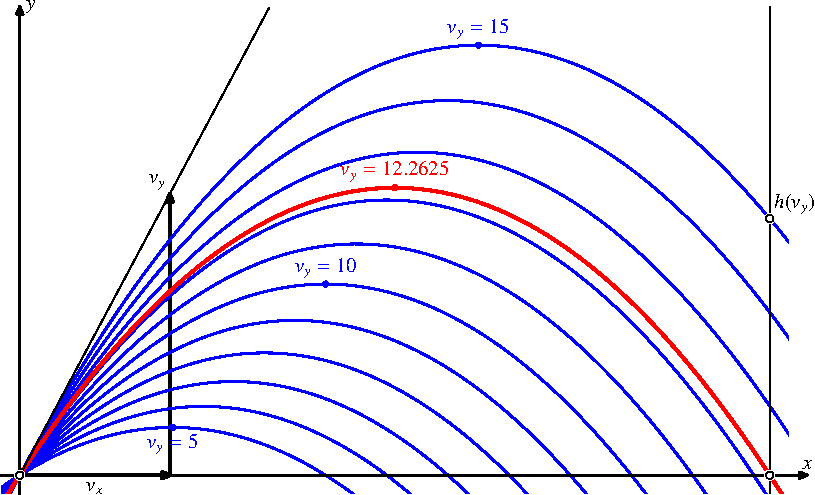
\includegraphics{chapters/images/randwert-1.pdf}
\caption{L"osungen des Anfangswertproblems~(\ref{numerik:ball-dgl-1}) und
(\ref{numerik:ball-dgl-2}).
Das Newton-Verfahren korrigiert $v_y$ derart, dass $y(v_y)=0$ wird.
So wird die L"osung des Randwertproblems (rot) gefunden.
\label{numerik:randwert-bild}}
\end{figure}
Wir f"uhren den eben skizzierten Algorithmus f"ur das Ball-Problem durch.
Um die Jacobi-Matrix zu berechnen, m"ussen wir die Ableitung von $f$ berechnen:
\begin{equation}
\frac{\partial f(x,y)}{\partial y}
=
\begin{pmatrix}
0& 0& 1& 0\\
0& 0& 0& 1\\
0& 0& 0& 0\\
0& 0& 0& 0
\end{pmatrix}.
\end{equation}
Da die rechte Seite nicht von $y$ abh"angt, k"onnen wir die Gleichung f"ur
die Jacobi-Matrix ganz unabh"angig von $y$ l"osen.
Da $F$ so einfach ist, kann man das Matrizenprodukt direkt ausrechnen, 
so wird die Differentialgleichung f"ur $J$
\begin{equation}
\begin{pmatrix}
J'_{11}&J'_{12}&J'_{13}&J'_{14}\\
J'_{21}&J'_{22}&J'_{23}&J'_{24}\\
J'_{31}&J'_{32}&J'_{33}&J'_{34}\\
J'_{41}&J'_{42}&J'_{43}&J'_{44}
\end{pmatrix}
=
\begin{pmatrix}
0& 0& 1& 0\\
0& 0& 0& 1\\
0& 0& 0& 0\\
0& 0& 0& 0
\end{pmatrix}
\begin{pmatrix}
J_{11}&J_{12}&J_{13}&J_{14}\\
J_{21}&J_{22}&J_{23}&J_{24}\\
J_{31}&J_{32}&J_{33}&J_{34}\\
J_{41}&J_{42}&J_{43}&J_{44}
\end{pmatrix}
=
\begin{pmatrix}
J_{31}&J_{32}&J_{33}&J_{34}\\
J_{41}&J_{42}&J_{43}&J_{44}\\
     0&     0&     0&     0\\
     0&     0&     0&     0
\end{pmatrix}
\end{equation}
\begin{table}
\centering
\begin{tabular}{|>{$}r<{$}|>{$}r<{$}|>{$}r<{$}|>{$}r<{$}|>{$}r<{$}|>{$}r<{$}|>{$}r<{$}|>{$}r<{$}|}
\hline
n&    v_y&    t& x(t)&      y(x)&\displaystyle\frac{\partial^{\mathstrut}y}{\partial v_y}&v_{y,\text{new}}&\Delta\\
\hline
0& 7.0000&  2.5& 20.0&-13.156250&  2.5& 12.26250000& -5.2625000000\\
1&12.2625&  2.5& 20.0& -0.000004&  2.5& 12.26250145& -0.0000014458\\
2&12.2625&  2.5& 20.0&  0.000000&  2.5& 12.26250143&  0.0000000204\\
\hline
\end{tabular}
\caption{Newton-Algorithmus f"ur das Ball-Problem, Resultate der numerischen
Rechnung.
$v_y$ wird in drei Schritten mit einer Genauigkeit von mehr als 10 Stellen
gefunden.
\label{numerik:newton-resultate}}
\end{table}%
Daraus kann man ablesen, dass die Elemente $J_{3j}$ und $J_{4j}$ sich
nicht "andern, sie bleiben also konstant.
Aber auch in den ersten zwei Zeilen k"onnen sich nur die Elemente $J_{13}$
und $J_{24}$ "andern, die Differentialgleichungen f"ur diese Elemente
sind
\begin{align*}
J'_{13}&=1\\
J'_{24}&=1
\end{align*}
oder in Matrixform:
\begin{equation}
J(x) = \begin{pmatrix}
1&0&x&0\\
0&1&0&x\\
0&0&1&0\\
0&0&0&1
\end{pmatrix}
\end{equation}
Die L"osung $J_{13}(x)=x$ und $J_{24}=x$.
Damit haben wir die n"otige Information, um den Newton-Algorithmus
durchzuf"uhren.
In Tabelle~\ref{numerik:newton-resultate}
sind die Resultate der numerischen Rechnung zusammengestellt.
Es zeigt sich, dass der korrekte Wert f"ur $v_y$ in drei Iterationen
mit 10 Stellen Genauigkeit gefunden werden kann.
Damit ist das Randwertproblem numerisch gel"ost.
\end{beispiel}

\subsection{Finite Elemente}



